\begin{frame}[plain]% The optional argument 'plain' hides the headline and footline
	\begin{center}\bfseries\centering
		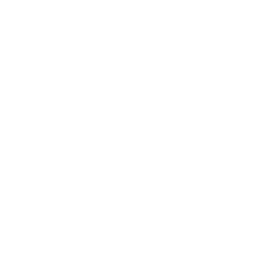
\includegraphics[scale=1]{Feathergraphics/cse_logo_opa0}
%		\includegraphics[scale=1]{\; \;}
		\vspace{-5.75cm} \\
		{\adjustbox{scale=3}{\color{cseblue} I. What is a Vector Field?}}
		\bigskip\bigskip % Vertical whitespace
		{\ }\vspace{4cm}\\
		\bigskip
	\end{center}
\end{frame}

\begin{frame}[fragile]{\textbf{I. What is a Vector Field?}}{Example}
\begin{center}
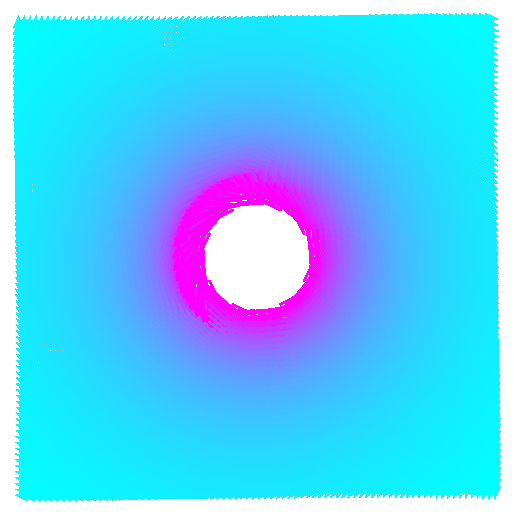
\includegraphics[scale=.9]{tikzs/vector-field2.pdf}
\end{center}
\end{frame}

\begin{frame}[fragile]{\textbf{I. What is a Vector Field?}}{Example}
\begin{center}
\begin{minipage}{.4\textwidth}
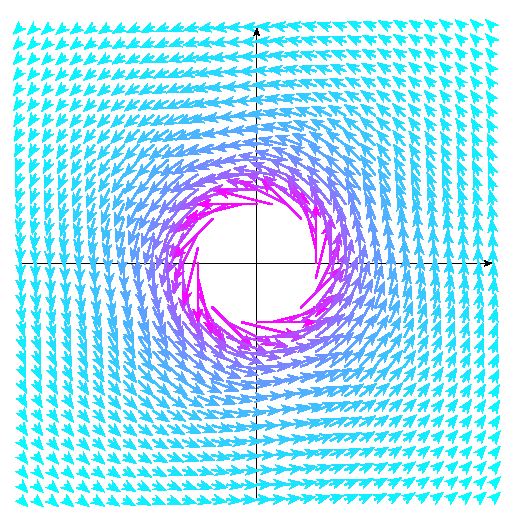
\includegraphics[scale=.8]{tikzs/vector-field1.pdf}\quad
\end{minipage}\hfill
\begin{minipage}{.5\textwidth}
Consider
\begin{align*}
\mathbf{F}(x,y)&=\begin{bmatrix}
	\displaystyle\frac{-y}{x^2+y^2}\\ \\ \displaystyle\frac{x}{x^2+y^2}
\end{bmatrix}=\begin{bmatrix}
	\displaystyle \frac{\partial}{\partial x}\theta\\ \\ \displaystyle\frac{\partial}{\partial y}\theta
\end{bmatrix}
\end{align*}
with $\theta=\theta(x,y)=\arctan(y/x)$.	
\end{minipage}
\end{center}
\end{frame}

\begin{frame}[fragile]{\textbf{I. What is a Vector Field?}}{Tangent space $T_pS^1$ (at a point $p\in S^1$)}
\begin{center}
\begin{minipage}{.3\textwidth}
	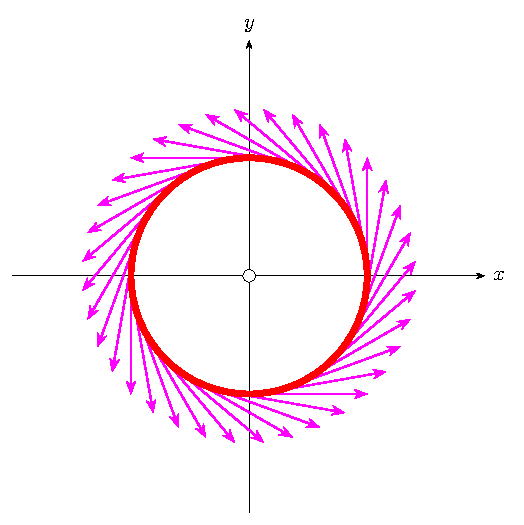
\includegraphics[scale=.5]{tikzs/vector-field3.pdf}\quad
\end{minipage}\hfill
\begin{minipage}{.6\textwidth}
Let \[
S^1:=\{(x,y)\in\mathbb R^2:x^2+y^2=1\}.
\] and consider the vector field \[
\vec{F}(x,y)=\begin{bmatrix}
	-y\\ x
\end{bmatrix}=\begin{bmatrix}
0 & -1 \\ 1 & 0
\end{bmatrix}\begin{bmatrix}
x \\ y
\end{bmatrix}.
\] Then \[
T_pS^1=\textrm{span}\left(\begin{bmatrix}
	-y\\ x
\end{bmatrix}\right).
\]
\end{minipage}
\end{center}
\vfill
\textbf{Note.}\; Fix $p\in S^1$. $T_pS^1$ is a one-dimensional line through the origin, spanned by $\vec{F}(p)$.
\end{frame}


\begin{frame}[fragile]{\textbf{I. What is a Vector Field?}}{Definition of a Vector Field with Tangent Space}
Define \[
TS^1:=\bigsqcup_{p\in S^1}T_pS^1=\set{(p,\vec{v}):p\in S^1, \vec{v}\in T_pS^1}.
\]
A \textbf{vector field} (on $S^1$) is a map \[
\fullfunction{\vec{X}}{S^1}{TS^1}{p}{(p,\vec{X}(p))},
\] where $\vec{X}(p)\in T_pS^1$.
\end{frame}


%Great—let’s build the objects **from the unit circle itself** and only then name them.
%
%# 1) Tangent space $T_pS^1$ (at a concrete point $p\in S^1$)
%
%Let $S^1=\{(x,y)\in\mathbb R^2:x^2+y^2=1\}$. Fix $p=(x,y)\in S^1$. Consider the constraint
%
%$$
%g:\mathbb R^2\to\mathbb R,\qquad g(u,v)=u^2+v^2-1.
%$$
%
%A velocity vector $v\in\mathbb R^2$ is tangent to $S^1$ at $p$ iff it is the derivative at $0$ of some curve $\gamma$ with $\gamma(0)=p$ and $g(\gamma(t))\equiv 0$; differentiating gives
%
%$$
%0=\tfrac{d}{dt}\,g(\gamma(t))\big|_{t=0}=Dg(p)\,v=2\langle p,v\rangle.
%$$
%
%Hence
%
%$$
%\boxed{\,T_pS^1=\{v\in\mathbb R^2:\ \langle p,v\rangle=0\}\,}
%$$
%
%i.e. the **tangent line** at $p$ is the line through the origin perpendicular to $p$. (For a 1-manifold each point carries a tangent **line**; here it is realized explicitly in $\mathbb R^2$.)&#x20;
%
%A convenient basis vector is the quarter-turn of $p$:
%
%$$
%J=\begin{pmatrix}0&-1\\[2pt]1&0\end{pmatrix},\qquad T(p):=Jp=(-y,x)\in T_pS^1,
%$$
%
%so $T_pS^1=\operatorname{span}\{(-y,x)\}$. (This vector is indeed tangent to the circle at every point.)&#x20;
%
%# 2) The tangent bundle as a **disjoint union** (bigsqcupuct of fibers)
%
%The **tangent bundle** of $S^1$ is the fiberwise disjoint union
%
%$$
%\boxed{\,TS^1\;=\;\bigsqcup_{p\in S^1}T_pS^1\;=\;\{(p,v)\in S^1\times\mathbb R^2:\ \langle p,v\rangle=0\}\,}
%$$
%
%with bundle projection $\pi:TS^1\to S^1$, $\pi(p,v)=p$. A (smooth) **vector field** is a smooth **section**
%
%$$
%X:S^1\longrightarrow TS^1,\qquad \pi\circ X=\mathrm{id}_{S^1}.
%$$
%
%(“Vector fields are smooth sections of the tangent bundle.”)&#x20;
%
%# 3) Your field, restricted to $S^1$, as a section $X:S^1\to \bigsqcup_{p}T_pS^1$
%
%Start from
%
%$$
%\vec F(u,v)=\Big(-\frac{v}{u^2+v^2},\,\frac{u}{u^2+v^2}\Big).
%$$
%
%On $S^1$ we have $u^2+v^2=1$, so $\vec F|_{S^1}(x,y)=(-y,x)=T(p)\in T_pS^1$. Thus the **section**
%
%$$
%\boxed{\,X:\ p=(x,y)\ \longmapsto\ \big(p,\;(-y,x)\big)\ \in T_pS^1\subset TS^1\,}
%$$
%
%is well defined and smooth; in angle coordinates $c(\theta)=(\cos\theta,\sin\theta)$,
%
%$$
%X\big(c(\theta)\big)=\big(c(\theta),\,(-\sin\theta,\cos\theta)\big)=\big(c(\theta),\,c_*\partial_\theta\big),
%$$
%
%i.e. the unit tangent field along the circle. (This matches the standard “vector field as section” formulation.)  &#x20;
%
%---
%
%### Micro-summary (all within the example)
%
%* $T_pS^1=\{v:\langle p,v\rangle=0\}$ is the tangent **line** at $p$.&#x20;
%* $TS^1=\bigsqcup_{p}T_pS^1=\{(p,v):\langle p,v\rangle=0\}$ with $\pi(p,v)=p$. Vector fields are smooth sections $X:S^1\to TS^1$.&#x20;
%* Your field restricts to $X(p)=(p,(-y,x))$, the standard unit tangent along $S^1$.&#x20;
